% Created 2020-12-08 Tue 10:40
% Intended LaTeX compiler: pdflatex
\documentclass[11pt]{article}
\usepackage[utf8]{inputenc}
\usepackage[T1]{fontenc}
\usepackage{graphicx}
\usepackage{grffile}
\usepackage{longtable}
\usepackage{wrapfig}
\usepackage{rotating}
\usepackage[normalem]{ulem}
\usepackage{amsmath}
\usepackage{textcomp}
\usepackage{amssymb}
\usepackage{capt-of}
\usepackage{hyperref}
\author{Dean Carmi}
\date{\today}
\title{Lab Report DDOS}
\hypersetup{
 pdfauthor={Dean Carmi},
 pdftitle={Lab Report DDOS},
 pdfkeywords={},
 pdfsubject={},
 pdfcreator={Emacs 27.1 (Org mode 9.5)}, 
 pdflang={English}}
\begin{document}

\maketitle
\tableofcontents


\section{Setting up the machines}
\label{sec:orgcfe95e3}
In order to do recreate the conditions of the experiment I included the instructions for each machine.
\subsection{Victim}
\label{sec:org66a739f}
The victim should include only a running \emph{apache server}, listening on port 80 (without firewall) 
\subsection{Monitor}
\label{sec:orga4b1b25}
In directory \texttt{monitor\_files} we have all files related to the monitor.
Using the \texttt{makefile} in that directory, steps to setup the system:
\begin{description}
\item[{\texttt{make hping}}] install nessecary package.
\item[{\texttt{make python\_scapy}}] installing everything related to the right version of python.
\end{description}
\subsection{Attacker}
\label{sec:org6b260a3}
In directory \texttt{attacker\_files} we have all files related to the attacker.
Using the \texttt{makefile} in that directory, steps to setup the system:
\begin{description}
\item[{\texttt{make python\_setup}}] install anything related to python.
\end{description}

\section{Creating the attack}
\label{sec:org437663b}
\subsection{Using C}
\label{sec:orgf620b29}
Instructions:
\begin{description}
\item[{Victim}] Run the apache server.
\item[{Attacker}] In directory \texttt{attacker\_files} run: 
\begin{itemize}
\item Compile - \texttt{make c\_ddos}
\item Run - \texttt{sudo ./syn\_flood 10.0.2.12 80} (You can replace the IP for any IP that you attack)
\end{itemize}
\item[{Monitor}] In directory \texttt{monitor\_files} run:
\begin{itemize}
\item Ping - \texttt{make start\_c} . \textbf{Note: You need to stop manually this process}
\end{itemize}
\end{description}
\subsubsection{After the attack}
\label{sec:orge8d9cc2}
\begin{description}
\item[{Attacker side}] A new file named \texttt{syns\_results\_c} will be created containing the required info.
\item[{Monitor side}] A new file named \texttt{pings\_results\_c\_raw.txt} will be created and we need to parse it. Run \texttt{python3.8 parse\_hping.py pings\_results\_c\_raw.txt}.
The script will ask you in which language the code is, you should reply \textbf{c} for C and \textbf{p} for Python. \textbf{Note: the RTT is in milliseconds}.
\end{description}
\subsection{Using Python}
\label{sec:orgab0374d}
Instructions:
\begin{description}
\item[{Victim}] Run the apache server.
\item[{Attacker}] In directory \texttt{attacker\_files} run: 
\begin{itemize}
\item Run - \texttt{sudo python3.8 ddos.py 10.0.2.12 80 1000000} (You can replace the IP for any IP that you want to attack, the last nubmer is the amount of packet, a million)
\end{itemize}
\item[{Monitor}] In directory \emph{monitor\textsubscript{files}} run:
\begin{itemize}
\item Ping - \texttt{make start\_py} . \textbf{Note: You need to stop manually this process}
\end{itemize}
\end{description}
\subsubsection{After the attack}
\label{sec:org18c2761}
\begin{description}
\item[{Attacker side}] A new file named \texttt{syns\_results\_p} will be created containing the required info.
\item[{Monitor side}] A new file named \texttt{pings\_results\_p\_raw.txt} will be created and we need to parse it. Run \texttt{python3.8 parse\_hping.py pings\_results\_p\_raw.txt}.
The script will ask you in which language the code is, you should reply \textbf{c} for C and \textbf{p} for Python. \textbf{Note: the RTT is in milliseconds}
\end{description}
\section{Report}
\label{sec:orgd96f47b}
\subsection{Regarding \emph{syns results}}
\label{sec:org78d6638}
\begin{description}
\item[{C code}] 
\end{description}
\begin{figure}[htbp]
\centering
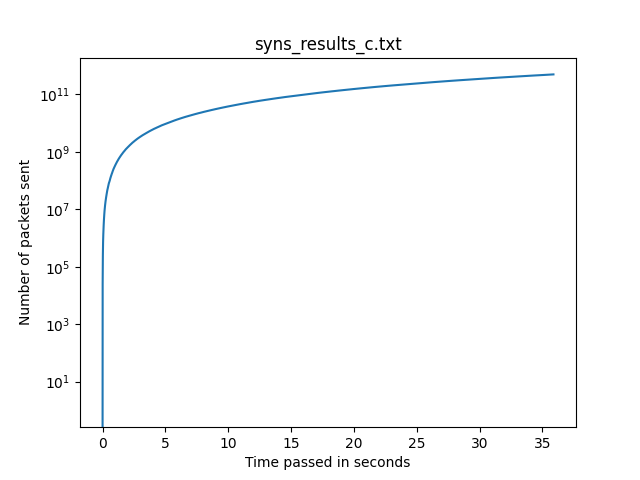
\includegraphics[width=.9\linewidth]{results/Syn_pkts_c.png}
\caption{Results of syn packet sending with C}
\end{figure}
\begin{itemize}
\item Average time for a packet - 0.000036 seconds.
\item Total running time - 52.894455 seconds.
\item Standard deviation - 0.0000315946680146141
\end{itemize}


\begin{description}
\item[{Python code}] 
\end{description}
\begin{figure}[htbp]
\centering
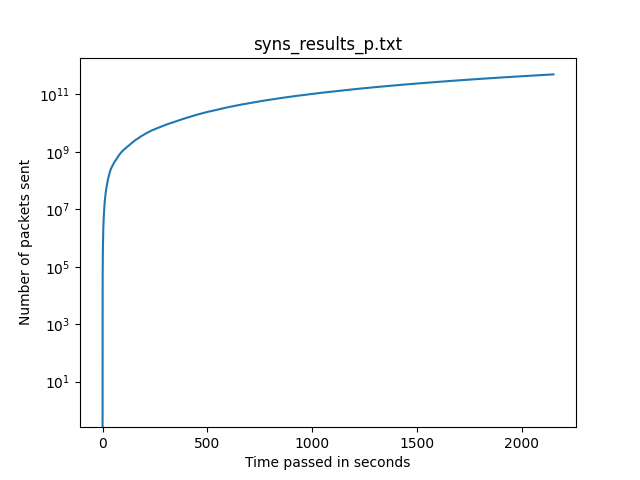
\includegraphics[width=.9\linewidth]{results/Syn_pkts_p.png}
\caption{Results of syn packet sending with Python}
\end{figure}
\begin{description}
\item[{Average time for a packet}] 0.002151517 seconds.
\item[{Total running time}] 2515.619506395 seconds.
\item[{Standard deviation}] 0.0004762834996620782
\end{description}
\subsubsection{Explaination}
\label{sec:org730e790}
We can observe two differences:
\begin{itemize}
\item Attack Time - C took 52 seconds vs Python that took 2515 seconds. C was faster by a factor of 48.
\item Average time for a packet - C took 0.000036 seconds vs Python that took 0.00215 seconds. Python was slower by a factor of 59.
\end{itemize}
We know that because Python is an interpreted language, it amplifies the number of actual CPU instructions required to perform the code given (compared to code in C).
In addition, In my case the Python code didn't run as machine code (like the C code), but it ran in a virtual machine (the bytecode interpreter).
\subsection{Regarding the \emph{pings results}}
\label{sec:orgebac00a}
\begin{description}
\item[{C code}] 
\end{description}
\begin{figure}[htbp]
\centering
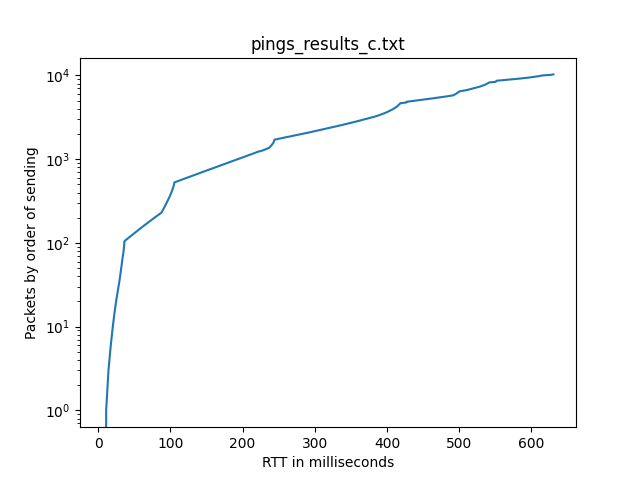
\includegraphics[width=.9\linewidth]{/home/dean/Documents/cyber-attack/ddos_assignment/results/Pings_c.png}
\caption{Results of the pings sending when the C attack took place}
\end{figure}
\begin{center}
\begin{tabular}{lr}
Average RTT & 4.378472 milliseconds\\
Standart deviation & 2.6498208\\
\end{tabular}
\end{center}

\begin{description}
\item[{Python code}] 
\end{description}
\begin{figure}[htbp]
\centering
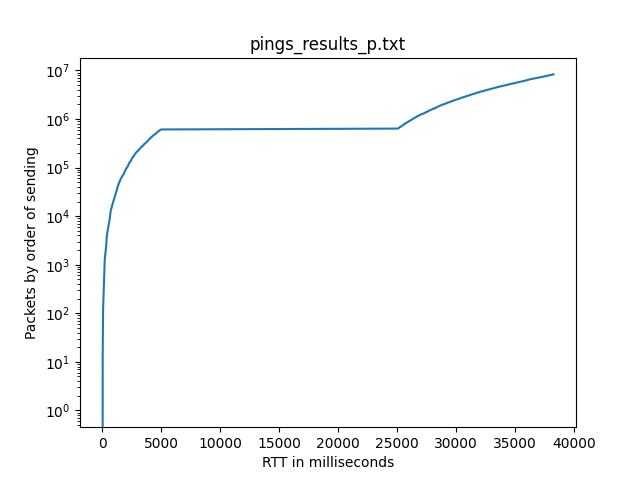
\includegraphics[width=.9\linewidth]{/home/dean/Documents/cyber-attack/ddos_assignment/results/Pings_p.png}
\caption{Results of the pings sending when the Python attack took place}
\end{figure}
\begin{center}
\begin{tabular}{lr}
Average RTT & 9.39337423 milliseconds\\
Standard deviation & 69.80985083\\
\end{tabular}
\end{center}
\subsubsection{Explaination}
\label{sec:org728755e}
\begin{itemize}
\item Average RTT
\end{itemize}
\end{document}
